% Źródła: materialy/2026-10-29/IMG_7044--IMG_7050.jpeg.
\chapter{Rozkłady zmiennych losowych}
\label{chap:rozklady-zmiennych-losowych}

\section{Rozkład prawdopodobieństwa}
\label{sec:rozklad-prawdopodobienstwa}

\begin{definicja}
\label{def:rozklad-prawdopodobienstwa}
\emph{Rozkładem prawdopodobieństwa na $\R^n$} nazywamy każdą miarę
probabilistyczną $\mu$ na przestrzeni mierzalnej $(\R^n,\B(\R^n))$,
czyli miarę taką, że $\mu(\R^n)=1$.
\end{definicja}

\begin{definicja}
\label{def:rozklad-zmiennej-losowej}
Niech $X\colon\Omega\to\R^n$ będzie wektorem losowym na przestrzeni
$(\Omega,\F,\PP)$. \emph{Rozkład zmiennej losowej $X$} to miara
$\mu_X$ określona wzorem
\[
  \mu_X(A)=\PP(X\in A)=\PP\bigl(X^{-1}(A)\bigr),
  \qquad A\in\B(\R^n).
\]
\end{definicja}

W szczególności
\[
  \mu_X(\R^n)=\PP(X\in\R^n)=\PP(\Omega)=1.
\]
Schemat przejścia od zdarzenia w przestrzeni wyników do zbioru wartości
zmiennej przedstawia rysunek~\ref{fig:schemat-rozkladu}.

\begin{figure}[H]
  \centering
  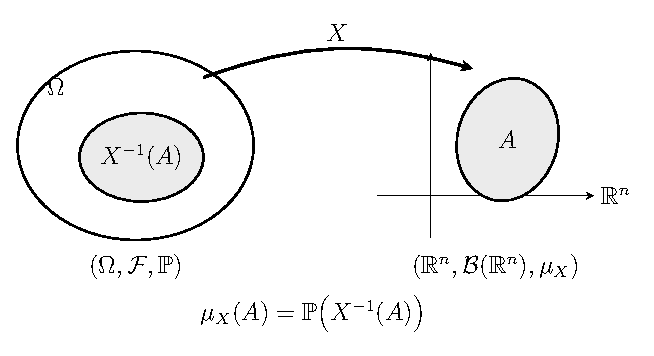
\includegraphics[width=10.5cm]{schemat-rozkladu.pdf}
  \caption{Zbiorowi borelowskiemu $A\subseteq\R^n$ odpowiada zdarzenie
    $X^{-1}(A)\subseteq\Omega$.
    Rozkład przypisuje mu masę $\mu_X(A)=\PP(X^{-1}(A))$.}
  \label{fig:schemat-rozkladu}
\end{figure}

\begin{przyklad}[Trzy zmienne na odcinku jednostkowym]
\label{przykl:trzy-rozklady}
Rozważmy przestrzeń probabilistyczną
\[
  (\Omega,\F,\PP)=\bigl([0,1],\B([0,1]),\lambda\bigr),
\]
gdzie $\lambda$ jest miarą Lebesgue'a na $[0,1]$.

\emph{a) Zmienna stała.} Niech $X(\omega)=c$ dla każdego $\omega\in[0,1]$,
gdzie $c\in\R$. Dla $A\in\B(\R)$ mamy
\[
  \mu_X(A)=\PP(X\in A)=
  \begin{cases}
    1,&c\in A,\\
    0,&c\notin A.
  \end{cases}
\]
Jest to \emph{miara Diraca w punkcie $c$}, oznaczana przez $\delta_c$.

\emph{b) Indykator.} Niech
\[
  Y(\omega)=\mathbf{1}_{[0,\,2/3)}(\omega).
\]
Wówczas dla każdego $A\in\B(\R)$
\[
  \mu_Y(A)=
  \begin{cases}
    1,&0\in A,\ 1\in A,\\[2pt]
    \dfrac13,&0\in A,\ 1\notin A,\\[5pt]
    \dfrac23,&0\notin A,\ 1\in A,\\[5pt]
    0,&0\notin A,\ 1\notin A.
  \end{cases}
\]
Możemy zatem zapisać
\[
  \mu_Y=\frac13\delta_0+\frac23\delta_1.
\]

\emph{c) Zmienna identycznościowa.} Dla $Z(\omega)=\omega$, $\omega\in[0,1]$,
otrzymujemy
\[
  \mu_Z(A)=\PP(Z\in A)=\lambda\bigl([0,1]\cap A\bigr),
  \qquad A\in\B(\R).
\]
Wykresy zmiennych z tego przykładu pokazano na
rysunku~\ref{fig:trzy-zmienne}.
\end{przyklad}

\begin{figure}[H]
  \centering
  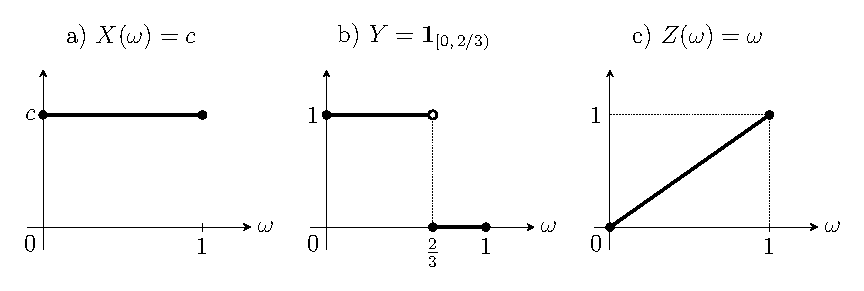
\includegraphics[width=\textwidth]{przyklady-zmiennych.pdf}
  \caption{Wykresy trzech zmiennych z przykładu~\ref{przykl:trzy-rozklady}.
    Są to wykresy funkcji na $\Omega=[0,1]$.}
  \label{fig:trzy-zmienne}
\end{figure}

\begin{przyklad}[Liczba szóstek]
\label{przykl:rozklad-liczby-szostek}
Rzucamy niezależnie $n$ razy uczciwą kostką. Niech $X$ oznacza liczbę
szóstek w tych rzutach. Wówczas
\[
  \mu_X(\{k\})=\PP(X=k)
    =\binom nk\left(\frac16\right)^k\left(\frac56\right)^{n-k},
  \qquad k=0,1,\ldots,n.
\]
Zmienna $X$ nie przyjmuje innych wartości, więc na przykład
\[
  \mu_X\!\left(\left\{\frac32\right\}\right)=0,
  \qquad \mu_X(\{n+1\})=0.
\]
Dla dowolnego $A\in\B(\R)$ mamy
\begin{align*}
  \mu_X(A)
    &=\sum_{k=0}^n\PP(X=k)\delta_k(A)\\
    &=\sum_{k=0}^n\binom nk
      \left(\frac16\right)^k\left(\frac56\right)^{n-k}\delta_k(A).
\end{align*}
\end{przyklad}

\section{Rozkłady dyskretne}
\label{sec:rozklady-dyskretne}

\begin{definicja}
\label{def:rozklad-dyskretny}
Niech $X\colon\Omega\to\R$ będzie zmienną losową. Definiujemy
\[
  S_X=\{x\in\R:\mu_X(\{x\})=\PP(X=x)>0\}.
\]
Mówimy, że $X$ ma \emph{rozkład dyskretny}, jeżeli
\[
  \PP(X\in S_X)=1.
\]
\end{definicja}

\begin{uwaga}
Mówimy, że rozkład zmiennej $X$ jest \emph{skupiony na zbiorze $A$},
jeżeli $A\in\B(\R)$ oraz $\PP(X\in A)=1$.
\end{uwaga}

\begin{fakt}
\label{fakt:przeliczalnosc-atomow}
Zbiór $S_X$ jest co najwyżej przeliczalny.
\end{fakt}
\noindent\emph{Dowód pozostawiono jako ćwiczenie.}

\begin{fakt}
\label{fakt:opis-rozkladu-dyskretnego}
Rozkład dyskretny jest jednoznacznie wyznaczony przez zbiór
\[
  S_X=\{x_n:n\in T\},
\]
gdzie $T$ jest co najwyżej przeliczalnym zbiorem indeksów, punkty $x_n$
są różne, oraz przez liczby
\[
  p_n=\PP(X=x_n),\qquad n\in T.
\]
Wówczas
\[
  \sum_{n\in T}p_n=1,
  \qquad
  \mu_X(A)=\PP(X\in A)=\sum_{\substack{n\in T\\x_n\in A}}p_n,
  \quad A\in\B(\R).
\]
\end{fakt}

\subsection{Przykłady rozkładów dyskretnych}
\label{subsec:przyklady-rozkladow-dyskretnych}

\begin{przyklad}[Rozkład skupiony w jednym punkcie]
Dla $a\in\R$ rozkład $\mu=\delta_a$ spełnia
\[
  \mu(A)=\delta_a(A),\qquad A\in\B(\R).
\]
Zmienna o tym rozkładzie spełnia $\PP(X=a)=1$.
\end{przyklad}

\begin{przyklad}[Rozkład dwupunktowy]
Niech $p\in[0,1]$ oraz $q=1-p$. Jeżeli
\[
  \PP(X=1)=p,\qquad\PP(X=0)=q,
\]
to
\[
  \mu_X=p\delta_1+(1-p)\delta_0.
\]
Ogólniej, rozkład skupiony na dwóch różnych punktach $x_1,x_2$ ma postać
$\alpha\delta_{x_1}+(1-\alpha)\delta_{x_2}$ dla pewnego $\alpha\in[0,1]$.
\end{przyklad}

\begin{przyklad}[Rozkład Bernoulliego]
\label{przykl:rozklad-bernoulliego}
Rozkład Bernoulliego $B(n,p)$, gdzie $n\geq1$ i $p\in[0,1]$,
jest określony przez
\[
  \PP(X=k)=\binom nk p^k(1-p)^{n-k},
  \qquad k=0,1,\ldots,n.
\]
W przypadkach brzegowych stosujemy konwencję $0^0=1$.
\end{przyklad}

\begin{przyklad}[Rozkład geometryczny]
\label{przykl:rozklad-geometryczny}
Dla $p\in(0,1]$ rozkład geometryczny, oznaczany przez $G(p)$,
jest dany wzorem
\[
  \PP(X=k)=(1-p)^{k-1}p,\qquad k=1,2,\ldots.
\]
Piszemy wówczas $X\sim G(p)$; dla $p=1$ cała masa jest skupiona w punkcie $1$.
\end{przyklad}

\begin{przyklad}[Rozkład Poissona]
\label{przykl:rozklad-poissona}
Rozkład Poissona o parametrze $\lambda\geq0$, oznaczany przez
$\operatorname{Pois}(\lambda)$, jest określony przez
\[
  \PP(X=k)=\frac{\lambda^k}{k!}e^{-\lambda},
  \qquad k=0,1,2,\ldots.
\]
Piszemy $X\sim\operatorname{Pois}(\lambda)$.
Dla $\lambda=0$ rozkład jest równy $\delta_0$.
\end{przyklad}
